\documentclass[journal,10pt,twocolumn]{article}
\usepackage{graphicx, float}
\usepackage[margin=0.5in]{geometry}
\usepackage{amsmath, bm}
\usepackage{array}
\usepackage{booktabs}

\providecommand{\norm}[1]{\left\lVert#1\right\rVert}
\let\vec\mathbf
\newcommand{\myvec}[1]{\ensuremath{\begin{pmatrix}#1\end{pmatrix}}}
\newcommand{\mydet}[1]{\ensuremath{\begin{vmatrix}#1\end{vmatrix}}}

\title{\textbf{Circle Assignment}}
\author{P Pavan Kumar}
\date{October 2022}

\begin{document}

\maketitle
\paragraph{\textit{Problem Statement} - let $ 2x^2+y^2-3xy=0 $ equation of a pair of tangents drawn from the origin O to a circle of radius 3 with centre in the first quadrant. If A is one of the points of contact, find the length of OA..}

\section*{\large Figure}

\begin{figure}[H]
\centering
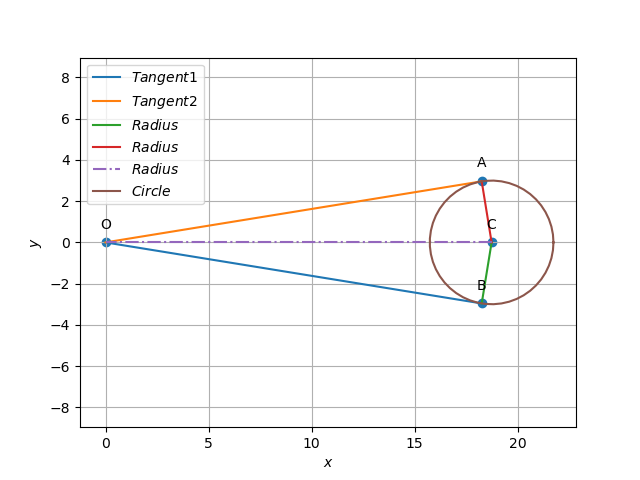
\includegraphics[width=1\columnwidth]{circle.png}
\caption{length of OA = 18.728}
\label{fig:triangle}
\end{figure}
\section*{\large Solution}
The equation of the pair of tangents is $ 2x^2+y^2-3xy=0 $ and r=3.
\\The equation in quadratic form is 
 \begin{equation*}
   \vec{  x^Tvx + 2u^Tx}+f=0
 \end{equation*}
 from above v,u,f are
 \begin{equation*}
 	\vec{v= \begin{pmatrix}
 				2&\frac{-3}{2}\\\frac{-3}{2}&1
 			 \end{pmatrix},
 			 u }= \myvec{0\\0},f=0
 \end{equation*}
 \hspace{40mm}$ \vec{x^Tvx} = 0 $\\
 \begin{equation*}
 \vec{v=P^TDP}
 \end{equation*}
 on solving we get $ \vec{\lambda_1,\lambda_2, P} $ 
\begin{equation*}
\lambda_1 = 3.081,\hspace{1mm} \lambda_2 = -0.081,\hspace{1mm}P=\begin{pmatrix}
0.811&0.584\\-0.584&0.811
\end{pmatrix}
 \end{equation*}
 the pair of straight line can be expressd as
 \begin{equation*}
\vec{(\sqrt{|\lambda_1|}\hspace{2mm} \pm \sqrt{|\lambda_2})P^T(X-C)=0}  
 \end{equation*}
 where,
 \hspace{30mm}$ \vec{C=v^{-1}u} $\\\begin{equation*}
 \vec{C = 0 } 
 \end{equation*} 
the normal vectors of the lines are
\begin{equation*}
\vec{n_1 = P\myvec{\sqrt{\lambda_1}\\\sqrt{\lambda_2}}}
\end{equation*} 
\begin{equation*}
\vec{n_2 = P\myvec{\sqrt{\lambda_1}\\-\sqrt{\lambda_2}}}
\end{equation*} 
 on solving normal vectors are
 \begin{equation*}
    \vec{n_1} = \myvec{1.59\\-0.79},
     \vec{n_2} = \myvec{1.25\\-1.25}
 \end{equation*}
 the angle between the two vectors $ n_1 and n_2 $ is given by 
 \begin{equation*}
     cos\theta = \vec{\frac{n_1^Tn_2}{\|n_1\|\|n_2\|}}
 \end{equation*}
 \begin{equation*}
      \theta = \cos^{-1}\myvec{\vec{\frac{n_1^Tn_2}{\|n_1\|\|n_2\|}}}
 \end{equation*}
 
 \vspace{2mm}

\hspace{25mm} $ \theta = 18.434 $\\
to find the length of the OA 
\begin{equation*}
     OA = r*cosec\frac{\theta}{2}
\end{equation*}
on solving the length of OA
\begin{equation*}
    OA = 18.728
\end{equation*}

\end{document}